%%=============================================================================
%% Methodologie
%%=============================================================================

\chapter{\IfLanguageName{dutch}{Methodologie}{Methodology}}
\label{ch:methodologie}
In het vorige hoofdstuk werd een overzicht gegeven van theoretische software oplossingen die het mogelijk maken voor een organisatie om beter te voldoen aan de GDPR. Dit hoofdstuk zet dit in de praktijk om door een organisatie (InSites Consulting) te analyseren, te bekijken welke oplossingen reeds in plaats zijn, en wat nog beter kan. 
Er is een opnieuw een groot deel gewijd aan het extraheren van persoonlijke data uit foto's en tekst door middel van Machine Learning. 

\section{InSites Consulting}
InSites Consulting is een marktonderzoeksbureau (met ongeveer 300 werknemers verspreid over 7 landen). InSites onderzoekt op basis van opdrachten van klanten waarom bepaalde producten minder/beter scoren, hoe populair een bepaald merk is, enzoverder. Hiervoor wordt zowel kwantitatief als kwalitatief onderzoek uitgevoerd op een brede groep van respondenten, wereldwijd. Bijgevolg komt InSites in \textbf{grote mate in contact met persoonlijke informatie}. 

\section{Controlelijst software-oplossingen} 
Een eerste stap bij het praktisch onderzoeken naar welke verbeteringen een bedrijf gdpr-gewijs kan uitvoeren, is een overzicht opstellen. Een overzicht van wat reeds in plaats is, en welke werkpunten er nog zijn. Deze controlelijst is toegepast op InSites Consulting, maar kan gebruikt worden voor elke organisatie die op grote basis gegevens verwerkt, en op zoek is naar software oplossingen om die gegevens te beschermen. 

In de eerste kolom staan de onderwerpen die software oplossingen voor de GDPR voorstellen. Een vinkje in tweede kolom betekent dat InSites dit reeds op een goede manier geïmplementeerd heeft. Een vinkje in de derde kolom betekent dat dit onderwerp nog niet in plaats is/ nog kan verbeterd worden. Alle onderwerpen zijn in 'stand van zaken' in algemene vorm uitgelegd, en worden verder in dit onderzoek specifiek voor InSites Consulting geëvalueerd. 

TABEL NOG UP TE DATEN 

	\begin{tabularx}{\linewidth}{ |X|l|l| } 
		\hline
		Software oplossing om gdpr compliant te worden & Goed & Verbeter  \\ [0.5ex]
		
		\hline\hline
		\textbf{Privacy policy mededeling} & \checkmark &  \\ 
		Splash pages  &  &  \\ 
		beknopte, transparante, begrijpelijke en toegankelijke vorm  &  &  \\ 
		duidelijke en ondubbelzinnige taal  &  &  \\ 
		Gratis  & \checkmark &  \\ 
		Tijdig aangeboden worden.  &  &  \\ 
		\textbf{Data Retention} &  & \checkmark \\ 
		De juiste beweegredenen &  &  \\
		Actualisering van de gegevens  &  &  \\
		\hline
		Data Access Control &  & \checkmark \\ 
		\hline
		\textbf{Data Security} &  &  \\
		2-factor authentication  & \checkmark &  \\ 
		aanvullingen hier & \checkmark &  \\ 
		\hline
		Toestemming van de gebruiker?  & \checkmark &  \\ 
		\hline
		\textbf{Pseudo en anonimisatie} &  &  \\ 
		\hline
		\textbf{Rechten van de betrokkene} &  &  \\ 
		Mogelijkheid vraag tot verwijdering gegevens & \checkmark &  \\ 
		Anonimisering voor de hand liggende gegevens & \checkmark &  \\
		Anonimisering niet voor de hand liggende gegevens & & \checkmark  \\
		Data Security &  &  \\ 
		
		Privacy policy mededeling & \checkmark &  \\ 
		
		Data Security &  &  \\ 
		\hline
		
	\end{tabularx}

note to self: privacy policy mededeling samen met data retention, staat het erin hoe lang wordt bijgehouden etc? 


%\subsection{Data Protection}

%% TODO: Hoe ben je te werk gegaan? Verdeel je onderzoek in grote fasen, en
%% licht in elke fase toe welke stappen je gevolgd hebt. Verantwoord waarom je
%% op deze manier te werk gegaan bent. Je moet kunnen aantonen dat je de best
%% mogelijke manier toegepast hebt om een antwoord te vinden op de
%% onderzoeksvraag.
\section{Privacy Policy}

\section{Data retention}

Zoals beschreven in stand van zaken (2.2.3) is het belangrijk als organisatie een juiste beslissingen te maken hoe lang persoonlijke data zal worden bijgehouden. 

InSites Consulting krijgt elke dag enorme hoeveelheden aan data binnen, waarvan slechts een fractie als persoonlijke data kan worden aanzien. Oorspronkelijk, voor de GDPR, hielden ze alle data voor onbepaalde tijd bij. 

Een eerste stap die hier moet ondernomen worden is de persoonlijke data scheiden van andere data. Op deze manier kunnen ze verder gaan met het bijhouden van alle data die buiten de GDPR valt in welke mate ze zelf willen, en de data die wel persoonlijke informatie bevat binnen een bepaalde tijdspanne gaan verwijderen. 

Hoe is dit aangepakt? Eerst is het probleem gegeneraliseerd: het is niet nodig bij elke ingevulde vragenlijst elke vraag afzonderlijk te gaan beoordelen. 
Dit zou enkel tot nodeloos ingewikkelde implementaties leiden, met minimaal voordeligere resultaten. 

Daarom is het beslissingsniveau of data al dan niet persoonlijke info kan bevatten, op 'Activity'-niveau gelegd (een activity bij InSites Consulting is een kwantitatief of kwalitatief onderzoek, zoals een vragenlijst). Bij creatie van een Activity kan worden beslist of deze over persoonlijke onderwerpen zal gaan, en/of er een mogelijkheid zal zijn dat er data wordt ontvangen van participanten met persoonlijke informatie. 
Dit is op een eenvoudig wijze opgelost door middel van een 'checkbox' op de pagina waar de Activity wordt aangemaakt. (Zie figuur) NOTE TO SELF SCREENSHOT VAN SQUAREINFOPAGE 

Op deze manier kan in de databasetabel met info over de Activities een extra kolom worden toegevoegd: PII-sensitive; met een bit-waarde (0 bij niet persoonlijke info, 1 voor wel persoonlijke info). 
Dan kan, bij het bereiken van een bepaalde datum na creatie van deze Actvity, afhankelijk van de waarde binnen de PII-sensitive-tabel, een activity verwijderd worden. Hierbij worden alle gegevens, gehaald uit die Activity, mee verwijderd of geanonimiseerd. Dankzij deze oplossing (=de checkbox) kan dit geautomatiseerd gebeuren, en is er geen nood aan een werknemer die alles handmatig overloopt. 

\subsection{Data Access Control}
NOTE TO SELF KLEINE INLEIDING HIER 


Op bepaalde plaatsten binnnen de software van InSites Consulting is het voor admin users (=werknemers die marktonderzoek uitvoeren) mogelijk om exports te nemen van data. Deze exports worden dan in de vorm van een Excel-bestand lokaal opgeslagen bij werknemer.
Vaak bevat zo'n export persoonlijke data. Tenzij de data op de juiste manier beschermd is, en up-to-date wordt gehouden (wat niet het geval is bij InSites), voldoet dit niet aan de voorwaarden van de GDPR. 

\subsubsection{Bescherming}
Excel biedt zelf enkel oplossingen aan om data te beschermen (zie figuur 3.1). Een van de opties is om een excel bestand te beschermen met een \textbf{wachtwoord}. Dat lijkt misschien overbodig, aangezien enkel users met administrator rechten binnen InSites een export kunnen nemen, maar het biedt wel degelijk extra voordelen. Als je een wachtwoord instelt, blijft dit ook van kracht eens de worksheet gedownload is en lokaal opgeslagen staat. Zo heb je meer veiligheid in geval van een datalek waarbij data van persoonlijke pc's vrijgegeven is. Of wanneer iemand zijn wachtwoord is gelekt (bijvoorbeeld via phishing) om op de InSites-omgeving te graken. In dat geval zou de binnendringer wel de excel-sheet kunnen downloaden, maar de inhoud niet lezen. \\

Een aanvullende ingebouwd optie, \textbf{'Restrict Access'}, biedt de mogelijkheid om gebruikers bepaalde rechten (zoals data kopiëren) te ontnemen.IETS  MEER UITLEG HIER

\begin{figure}[h]
	\centering
	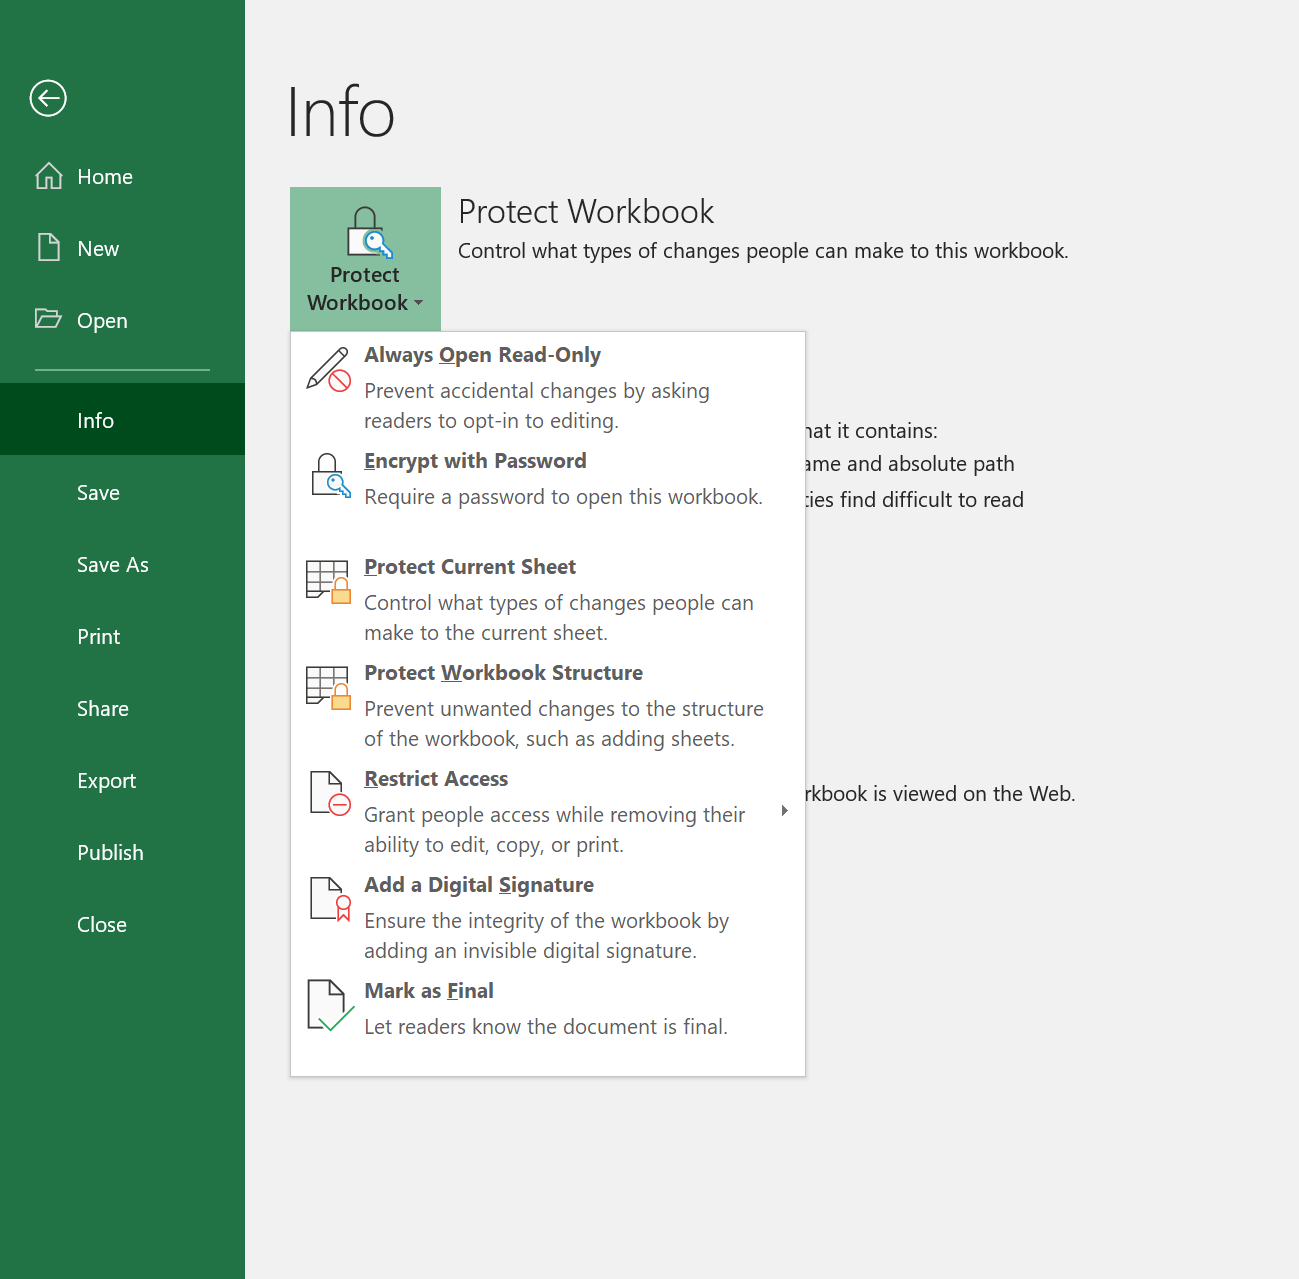
\includegraphics[width=\linewidth, scale=0.5]{Excel_beveiliging_opties}
	\label{fig:excelbeveiliging}
	\caption{Ingebouwde beveiligingsopties excel-worksheets.}
\end{figure}


\subsubsection{Logging en verwijdering}
LORET IPSUM. 

\subsubsection{Anonimisering}
 Dit is, om verscheidene eerder aangehaalde redenen, niet wenselijk. 
(foto hierin)

\section{Aanvraag tot verwijderen persoonlijke data}

Dit hoofdstuk zal ingaan op wat er kan gedaan worden wanneer een gebruiker een verzoek indient om al zijn persoonlijke data te verwijderen. 

\subsection{Mogelijkheid}
In de eerste plaats moet er een mogelijkheid zijn om deze aanvraag in de dienen. De manier waarop maakt weinig uit. Het kan door een knop op het platform/website/... ter beschikking te stellen als "Verwijder al mijn gegevens", waarna alles geautomatiseerd verwerkt wordt. Het kan ook door in je privacy policy mee te delen dat een mail kan gestuurd worden met deze aanvraag. De mogelijkheden zijn eindeloos. 

\subsection{Verwijdering voor de hand liggende gegevens}
Wanneer een aanvraag binnenkomt, kan een organisatie aan de slag. De eerste stap is om een overzicht te maken van waar alle data wordt bijgehouden, en te gaan bepalen welke data op welke plaatsen kan verwijderd worden. 


Met 'voor de hand liggende gegevens' wordt het volgende bedoeld: gegevens die specifiek zijn opgeslagen in de database, en worden aanzien al persoonlijke informatie. Denk aan voornaam en naam, telefoonnummer, adres, enzoverder. \\ 
Hier kan op eenduidige wijze een script worden opgesteld, dat de volledige database overloopt, en via een query al deze gegevens anonimiseert. Hiervoor zijn geen baanbrekende technologieën nodig en deze scripts zijn ook reeds in plaats bij InSites Consulting. Er zal dan ook niet verder worden op ingegaan tijdens dit inderzoek. 
 
\subsection{Verwijdering van niet voor de hand liggende gegevens}

In het geval van InSites Consulting (en dit zal ongetwijfeld ook voor veel andere organisaties gelden), bevat de verwerkte data veel meer persoonlijke elementen dan enkel de duidelijk identificeerbare velden zoals "naam". \\
Het bevat ook verborgen persoonlijke informatie zoals reacties op forumposts, antwoorden op vragenlijsten, enzoverder. De uitdaging is om ook dit geautomatiseerd als persoonlijke info te herkennen, zodat het kan verwijderd worden indien nodig. (zie stand van zaken 2.2.7)

In de volgende secties worden geautomatiseerde oplossingen te voorzien voor dit probleem. 
In stand van zaken werden hiervoor twee aanbieders uitgelicht, namelijk Microsoft Azure en Google cloud. In kader van de samenwerking met InSites Consulting is gekozen om de volgende applicaties uit te werken met Azure, aangezien InSites daar reeds klant is. Daarna is nog een hoofdstuk gewijd aan Google cloud voor extra technologieën. 

\subsection{Opzetten Azure omgeving}
in te vullen, reeds gebeurd, proces neerschrijven 


\subsection{ConsoleApplicatie PII uit text.}
In dit deel wordt een oplossing aangeboden voor het geautomatiseerd zoeken naar persoonlijke gegevens in tekst. 

Een goed startpunt om een applicatie op te zetten die gebruik maakt van Azure Cognitive Services is hun documentatie. 
bron % https://azure.microsoft.com/en-us/services/cognitive-services/
Hier wordt uitgelegd hoe je aan de slag kan om een applicatie te bouwen die requests stuurt naar de cognitive services-API. De mogelijkheden zijn eindeloos, maar de bedoeling in dit onderzoek is om geautomatiseerd stukken tekst uit een database te halen, deze te controleren op persoonlijke informatie, en zo nodig te verwijderen/ anonimiseren. 



\subsubsection{Stap 1: ConsoleApp die tekst inleest}
Cognitive services biedt voor Textanalyse een SDK aan.
 Deze sdk geeft toegang tot de verschillende cognitive services language API's, die zijn in staat tekst te analyseren en info uit te extraheren. In dit project is gekozen om te code te schrijven in C\# (een .NET project) omdat dit te voorkeur is van InSites Consulting. Microsoft biedt de SDK ook nog aan voor Python en Ruby. Als een onderneming geen gebruik wil maken van de aangeboden SDK, maar rechtstreeks API-calls wil uitvoeren, kan dit met GO, Java, Node.JS, PHP, Python of Ruby.\\

\begin{figure}[h]
	\centering
	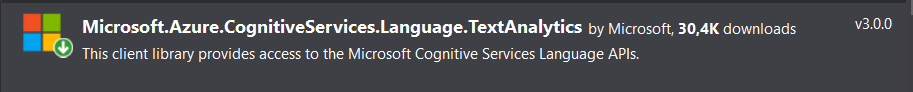
\includegraphics[width=\linewidth]{Ms_Cognitive_Services_TextAnalyticsSDK}
	\label{fig:textanalyticsSDK}
	\caption{SDK library van Microsoft die API's bevat voor tekstanalyse.}
\end{figure}

Wat de textanalyse-service aanbiedt is het herkennen van entiteiten in zinnen. In onderstaande tabel staat een overzicht van welke entiteiten worden ondersteund en kunnen worden herkend. 
https://docs.microsoft.com/en-us/azure/cognitive-services/text-analytics/how-tos/text-analytics-how-to-entity-linking
In de eerste kolom vindt je het type entiteiten, tweede kolom een voorbeeld, en in de derde kolom of deze entiteiten voor dit onderzoek interessant zijn: of ze al dan niet persoonlijke informatie bevatten. 

	\begin{tabularx}{\linewidth}{ |X|l|l| } 
	\hline
	Type & Voorbeeld & Mogelijk PII \\ [0.5ex]
	
	\hline\hline
	Persoon & Jeff & \checkmark \\ \hline 
	Locatie & 'Parijs', 'Redmond, Washington & \checkmark \\ \hline  
	Organisatie & Microsoft & \checkmark \\ \hline 
	Kwantiteit:Percentage, dimensie, temperatuur,... & 50\%, 10miles, ... & \\ \hline 
	Kwantiteit:Leeftijd & 30 years old & \checkmark \\ \hline 
	URL & www.bing.com & \checkmark \\ \hline 
	Email & test@test.com & \checkmark \\ \hline 
	Datum/tijd & 2nd may 2017 & \\ \hline 
	
	\hline
	
\end{tabularx}

De eerste stap is om een .NET-core project aan te maken (Console-app), en de Cognitive Services SDK te installeren.  
Daarna om van uit dit project  de API's van cognitive services aanspreken. In de eerste testfase werken we met mockdata. Je ziet in onderstaand codevoorbeeld enkele zinnen tekst. De bedoeling is deze zinnen te ontleden in entiteiten, en dan de gevonden entiteiten verder te beoordelen. 
Hiervoor wordt de data geanalyseerd door de EntitiesAsync-methode die ingebouwd is in de SDK. In onderstaand codevoorbeeld zijn de net omschreven stappen uitgewerkt in C\#. 

\begin{lstlisting}[frame=single]
var inputDocuments = new MultiLanguageBatchInput(
new List<MultiLanguageInput>
{
	new MultiLanguageInput("en", "1", "Microsoft was founded by Bill Gates and Paul Allen on April 4, 1975, to develop and sell BASIC interpreters for the Altair 8800."),
	new MultiLanguageInput("en", "3", "My emailadress is frederic.Terryn@hotmail.com"), 
	new MultiLanguageInput("en", "4", "Hi, @loredana16, do you like my picture?")
});
//...
var entitiesResult = await client.EntitiesAsync(false, inputDocuments);

// Printing recognized entities
foreach (var document in entitiesResult.Documents)
{
	Console.WriteLine($"Document ID: {document.Id} ");
	
	Console.WriteLine("\t Entities:");
	foreach (var entity in document.Entities)
	{
		Console.WriteLine($"\t\tName: {entity.Name},\tType: {entity.Type ?? "N/A"},\tSub-Type: {entity.SubType ?? "N/A"}");
		foreach (var match in entity.Matches)
		{
			Console.WriteLine($"\t\t\tOffset: {match.Offset},\tLength: {match.Length},\tScore: {match.EntityTypeScore:F3}");
		}
	}
}
\end{lstlisting}

\subsubsection{Stap 2: Analyseren mockdata}

Na het uitvoeren van bovenstaande methode, geeft de API een document terug met de herkende entiteiten. (Zie hieronder)
\begin{lstlisting}[frame=single]
Document ID: 1
Entities:
Name: Microsoft,        Type: Organization,     Sub-Type: N/A
Offset: 0,      Length: 9,      Score: 1,000
Name: Bill Gates,       Type: Person,   Sub-Type: N/A
Offset: 25,     Length: 10,     Score: 1,000
Name: Paul Allen,       Type: Person,   Sub-Type: N/A
Offset: 40,     Length: 10,     Score: 0,999
Name: April 4,  Type: Other,    Sub-Type: N/A
Offset: 54,     Length: 7,      Score: 0,800
Name: April 4, 1975,    Type: DateTime, Sub-Type: Date
Offset: 54,     Length: 13,     Score: 0,800
Name: BASIC,    Type: Other,    Sub-Type: N/A
Offset: 89,     Length: 5,      Score: 0,800
Name: Altair 8800,      Type: Other,    Sub-Type: N/A
Offset: 116,    Length: 11,     Score: 0,800
Document ID: 3
Entities:
Name: frederic.Terryn@hotmail.com,      Type: Email,    Sub-Type: N/A
Offset: 18,     Length: 27,     Score: 0,800
Document ID: 4
Entities:
\end{lstlisting}

In tabel ?? hebben we de bovenstaande codevoorbeelden samengesteld. In deze tabel kan je zien welke zin ontleed is en wat de service herkend heeft. Er wordt daarnaast getoond welke type entiteit herkend is, met welke zekerheid. 

\begin{tabularx}{\linewidth}{ |X|l|l|l| } 
	\hline
	Mockdata & Gevonden entiteit & Type & Zekerheid(\%)  \\ [0.5ex]
	
	\hline\hline
	"Microsoft was founded by Bill Gates and Paul Allen on April 4, 1975, to develop and sell BASIC interpreters for the Altair 8800".  & \begin{tabular}{@{}c@{}}
		Microsoft \\ Bill Gates \\ Paul Allen \\ April 4, 1975 \\ BASIC \\Altair 8800 \end{tabular} & 
	\begin{tabular}{@{}c@{}}
		Oranisation \\ Person \\ Person \\ DateTime \\ Other \\ Other  \end{tabular}
	& \begin{tabular}{@{}c@{}}
		100 \\ 100 \\ 99 \\ 80 \\ 80 \\ 80  \end{tabular}\\ 
	\hline\hline
		"My emailadress is frederic.Terryn@hotmail.com".  &
		\begin{tabular}{@{}c@{}}
			frederic.terryn \\ @hotmail.com  \end{tabular}  & 
		Email
	&  80\\ 
	\hline\hline
		"Hi, @loredana16, do you like my picture?".  &
	/  & 
	/
	&  / \\ 
	\hline
	
	
\end{tabularx}

In de eerste zin, een voorbeeldzin aangeboden in de documentatie Microsoft als voorbeeld, worden heel wat entiteiten herkend. 

In de tweede zin: "My emailadress is frederic.terryn@hotmail.com", wordt de inhoud meteen herkend als emailadres, met een zekerheidsscore van 0.8. Dit is dus alvast iets kan gebruikt worden, aangezien emailadressen als persoonlijke gegevens worden gezien, en deze dus in de toekomst kunnen gefiltert worden. 

De derde zin "Hi, @loredana16, do you like my picture?" is een test om te zien of het formaat van 'personentags', dat op zeer veel websites en forums gebruikt wordt, herkend wordt. Dit resultaat is negatief, er zijn geen entiteiten herkend in de derde zin. Dit betekent dus dat, als het formaat van tags moet gefiltert worden, dit niet automatisch via de basis-tekstanalyse zal kunnen


\subsubsection{Stap 3:handmatig filteren op niet herkende entiteiten}

\subsubsection{Stap 4: Mockdata vervangen door SQL database.}

\subsection{ConsoleApplicatie PII uit foto's.}
Naast tekst biedt Azure ook services aan om foto's te analyseren. De mogelijkheden hiervan zijn uitvoerig besproken in stand van zaken punt ?? . 

\subsubsection{Stap 1: ConsoleApp}

Eerst wordt getest in welke mate gezichten en entiteiten worden herkend op foto's. De voorbeeldfoto's in stand van zaken zijn demo-foto's aangeboden door Microsoft, dus deze geven geen betrouwbaar beeld. \\
Om dit te doen is de eerste stap opnieuw een \textbf{.NET console applicatie} te ontwikkelen, waarvoor een uitgebreide documentatie beschikbaar is op de website van Cognitive services. 
In de standaard-applicatie die microsoft aanbiedt moeten het pad naar een te analyseren foto handmatig ingevoerd worden. 
Dit is gewijzigd in de resulterende applicatie van dit onderzoek; er wordt gebruik gemaakt van een lijst van foto's: Mockdata. Deze Mockdata is 'hardcoded' toegevoegd aan het project. Wil een organisatie een SQL-database overlopen, kan dit eenvoudig zoals in Methodologie 3.4.5. 

In onderstaande codevoorbeeld vindt je de effectieve C\#-methode die de API van Microsoft aanroept en de foto analyseert. 

\begin{lstlisting}[frame=single]

static async Task MakeAnalysisRequest(string imageFilePath)
{
try
{
HttpClient client = new HttpClient();

client.DefaultRequestHeaders.Add(
"Ocp-Apim-Subscription-Key", subscriptionKey);

string requestParameters =
"visualFeatures=Categories,Description,Color";

string uri = uriBase + "?" + requestParameters;

HttpResponseMessage response;

byte[] byteData = GetImageAsByteArray(imageFilePath);

using (ByteArrayContent content = new ByteArrayContent(byteData))
{
content.Headers.ContentType =
new MediaTypeHeaderValue("application/octet-stream");

response = await client.PostAsync(uri, content);
}

string contentString = await response.Content.ReadAsStringAsync();

Console.WriteLine("\nResponse:\n\n{0}\n",
JToken.Parse(contentString).ToString());
}
catch (Exception e)
{
Console.WriteLine("\n" + e.Message);
}
}

static byte[] GetImageAsByteArray(string imageFilePath)
{
using (FileStream fileStream =
new FileStream(imageFilePath, FileMode.Open, FileAccess.Read))
{
BinaryReader binaryReader = new BinaryReader(fileStream);
return binaryReader.ReadBytes((int)fileStream.Length);
}
}

\end{lstlisting}

\subsubsection{Stap 2: Resultaten}
Deze methode maakt connectie met Cognitive services (er is dus een werkende internet verbinding nodig), en geeft zijn resulaten terug in JSON-formaat. 

De resultaten zijn opgedeeld in verschillende delen.\\ Als eerste wordt de foto aan een categorie toegekent. In het bovenstaande voorbeeld beslist de API dat de foto tot de \textbf{categorie} "people\_portrait" behoort. 

Daarna volgt een gedetailleerde beschrijving onder de vorm van \textbf{tags}. De eerste tags zoals 'person' en 'outdoor' zijn correct. Als we wat verder kijken in de lijst zien we enkele tags die niet bij de foto horen, zoals sunglasses, phone, en zelfs 'man'. 

Als laatste biedt de API nog een \textbf{conclusie-zin} aan die toont wat als hoofdelement op de foto herkend wordt. De zin 'a woman wearing glasses' is opvallend correct. 
De ander weergegeven info zoals formaat en dominante kleur zijn minder interessant binnen de scope van de GDPR.

\subsubsection{Stap 3: Resultaten gebruiken om PII-bevattende foto's te verwijderen.}
In deze stap is de applicatie verder ontwikkeld zodat hij niet langer toont welke informatie er in de foto's staat, maar aan de hand van deze informatie bepaalde foto's verwijdert. 

Dit gaat als volgt in z'n werk: Microsoft biedt \textbf{57 herkenbare categorieën} aan. Deze kunnen worden onderverdeeld in categoriën die mogelijk wijzen op aanwezigheid van persoonlijke info, en neutrale categorieën. Opgelet: dit is een eigen keuze voor elke onderneming die dit implementeert, veel categorieën zijn voor disucussie vatbaar. Bijvoorbeeld: alle categorieëen met 'Building'. Deze gebouwen kunnen huizen zijn, die dus verwijzen naar personen, of fabrieken die helemaal geen persoonlijke info bevatten. Op welke categorieën gefilterd wordt is dus een afweging die moet genomen worden. 
In dit onderzoek zijn volgende keuzes gemaakt: 

\textbf{Categorieën met mogelijk PII :}building\_, building\_arch, building\_brickwall, building\_church, building\_corner, building\_doorwindows, building\_pillar, building\_stair, building\_street, indoor\_, indoor\_churchwindow, indoor\_court, indoor\_doorwindows, indoor\_marketstore,
indoor\_room, 
,indoor\_venue \textbf{,people\_ ,people\_baby}
,people\_crowd
,people\_group
,people\_hand
,people\_many
,people\_portrait
,people\_show
,people\_tattoo
,people\_youngh
,people\_swimming
,text\_
,text\_mag
,text\_map
,text\_menu
,text\_sign
,outdoor\_pool ,trans\_bicycle

\textbf{Neutrale Categorieën:} abstract\_
,abstract\_net
,abstract\_nonphoto
,abstract\_rect
,abstract\_shape
,abstract\_texture
,animal\_
,animal\_bird
,animal\_cat
,animal\_dog
,animal\_horse
,animal\_panda
,dark\_
,drink\_
,drink\_can
,dark\_fire
,dark\_fireworks
,sky\_object
,food\_
,food\_bread
,food\_fastfood
,food\_grilled
,food\_pizza
,dark\_light
,others\_
,outdoor\_
,outdoor\_city
,outdoor\_field
,outdoor\_grass
,outdoor\_house
,outdoor\_mountain
,outdoor\_oceanbeach
,outdoor\_playground
,outdoor\_railway
,outdoor\_road
,outdoor\_sportsfield
,outdoor\_stonerock
,outdoor\_street
,outdoor\_water
,outdoor\_waterside
,plant\_
,plant\_branch
,plant\_flower
,plant\_leaves
,plant\_tree
,object\_screen
,object\_sculpture
,sky\_cloud
,sky\_sun

Dit is, binnen de applicatie, de \underline{eerste filter}. De input is een lijst met foto's.
Elke foto die door cognitive services wordt toegewezen aan een \textunderscore{categorie} van de eerste groep (categorie met mogelijk PII), wordt uit die lijst verwijderd. Hiermee zouden al alle foto's met mensen op moeten verwijderd zijn.

\subsubsection{stap 4: betrouwbaarheidstest}
Als test zijn 38 diverse foto's verzameld (zie bijlage voor alle foto's). Voornamelijk foto's van mensen in diverse situaties, met duidelijke/onduidelijke verlichting, achtergrond, enzoverder. 
Daarnaast zijn ook foto's geselecteerd van huizen en andere gebouwen. De bedoeling is om te vergelijken hoeveel van deze foto's door de applicatie herkend worden als persoonlijke informatie bevattend, ten opzichte van wat de schrijvers van dit onderzoek van mening zijn. f


Na interpretatie van de foto's krijgen we volgende resultaten: 
\begin{itemize}
	\item Foto's herkend als PII door onderzoeker: 27/40
	\item Foto's herkend als PII door applicatie: 22/40
\end{itemize}
Dit lijkt op het eerste zicht een vrij gelijklopende score. Maar als de resultaten beter bekeken worden blijkt dat er op verschillende foto's zijn aangeduid. (zie onderstaande tabel)

\begin{tabularx}{\linewidth}{ |l|l|l|X| } 
	\hline
	Fotonummer & PII-onderzoeker & PII-applicatie & Duidelijk fout  \\ [0.5ex]
	
	1 & Ja & Ja & \\
	2 & Ja & Ja & \\
	3 & Ja & Ja & \\
	4& Ja & Nee & Ja (kinderen) \\
	5& Ja & Nee & Ja (kind)\\
	6 & Ja & Ja & \\
	7 & Ja & Ja & \\
	8 & Ja & Nee & Ja(kinderen) \\
	9 & Ja & Ja & \\
	10 & Ja & Nee & Ja(kinderen) \\
	11 & Ja & Ja & \\
	12 & Ja & Ja & \\
	13 & Ja & Ja & \\
	14 & Nee & Nee & \\
	15 & Nee & Nee & \\
	16 & Ja & Nee & Ja \\
	17 & Ja & Ja & Nee  \\
	18 & Ja & Ja & \\
	19 & Ja & Nee & Ja \\
	20 & Ja & Ja & \\
	21 & Ja & Ja & \\
	22 & Ja & Ja & \\
	23 & Ja & Ja & \\
	24 & Ja & Ja & \\
	25 & Ja & Ja & \\
	26 & Ja & Ja & \\
	27 & Nee & Nee & \\
	28 & Ja & Nee & Nee\\
	29 & Nee & Nee & \\
	30 & Ja & Ja & \\
	31 & Nee & Ja & \\
	32 & Nee & Nee & \\
	33 & Ja & Ja & \\
	34 & Nee & Ja & \\
	35 & Nee & Nee & \\
	36 & Nee & Ja & Nee\\
	37 & Ja & Ja & \\
	38 & Ja & Nee & Ja \\
	\hline
	
\end{tabularx}

\subsubsection{stap 5: opkrikken betrouwbaarheidsniveau}
Het is duidelijk dat bij een aantal foto's de applicatie niet zegt: dit behoort tot een PII-categorie. Als dus enkel gefiltert wordt op zijn de resultaten niet betrouwbaar. De meest voorkomende fout is wanneer er mensen in beeld zijn, maar om allerhande redenen op iets onduidelijkere wijze. 

Een volgende stap is om te kijken of dit kan verbeterd worden. Daarvoor worden de JSON resultaten van de foto's die door de mens als PII herkend worden, maar niet door de applicatie, er bijgehaald. 

\begin{figure}[h]
	\centering
	\begin{subfigure}{0.45\textwidth}
		\centering
		
\includegraphics[width=.7\linewidth]{Fotosstest/2.jpg}
		\caption{Google cloud}
		\label{fig:qsdfqsdf}
	\end{subfigure}%
	\begin{subfigure}{0.45\textwidth}
		\centering
		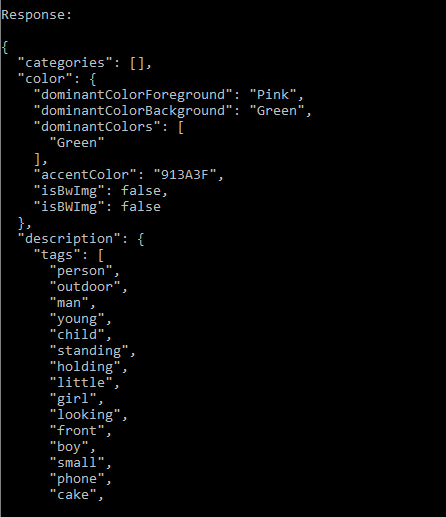
\includegraphics[width=.7\linewidth]{Fotosstest/2a.PNG}
		\caption{MS Cognitive Services.}
		\label{fig:sub2}
	\end{subfigure}
	\caption{Eenzelfde foto geïnterpreteerd door beide demo's. Google cloud herkent alle 3 de zichtbare gezichten, terwijl bij MS slechts één van de drie gezichten gevonden wordt.}
	\label{fig:teqsdfqsdfst}
\end{figure}

Cognitive services is er voor deze foto niet in geslaagd om een categorie toe te kennen aan de foto. Maar tussen de tags staat wel helemaal bovenaan: 'person'. Dit doet vermoeden dat wanneer er bijkomend op tags gefiltert wordt, er beter betrouwbare resultaten kunnen geboekt worden. 

Volgende tags worden toegevoegd als filter in de applicatie: 'person', 'child', 'young', 'man', 'girl', 'boy', 'girl'
Als nu een nieuwe betrouwbaardheidstest wordt gedaan krijgen we volgende resultaten: 
\begin{itemize}
	\item Foto's herkend als PII door onderzoeker: 27/40
	\item Foto's herkend als PII door applicatie: 34/40
\end{itemize}
ffkk

\begin{figure}[h]
	\centering
	\begin{subfigure}{0.45\textwidth}
		\centering
		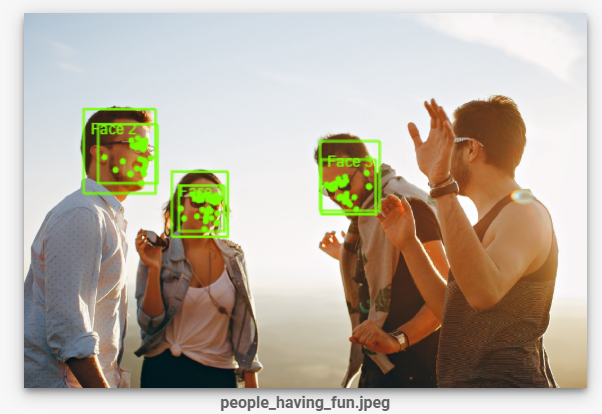
\includegraphics[width=.7\linewidth]{Face_recogn_google1.png}
		\caption{Google cloud}
		\label{fig:sub1}
	\end{subfigure}%
	\begin{subfigure}{0.45\textwidth}
		\centering
		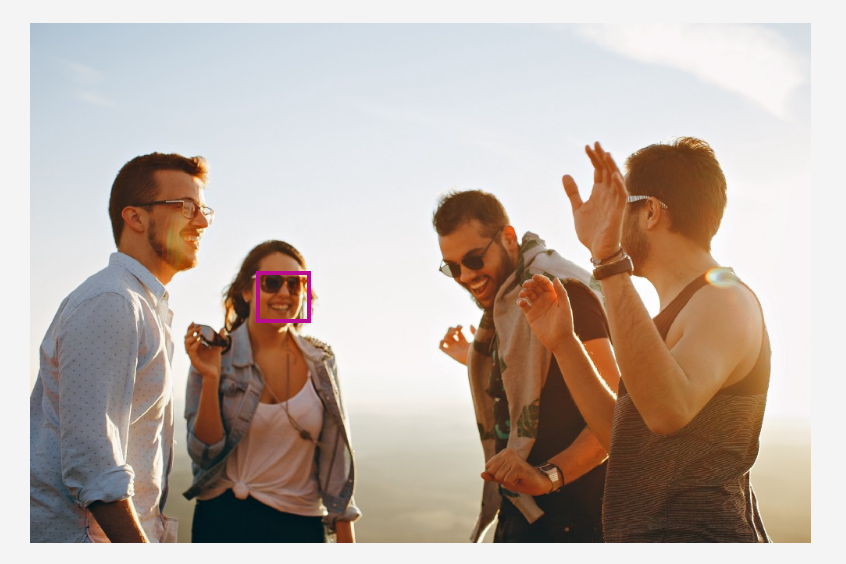
\includegraphics[width=.7\linewidth]{Face_recogn_micros_3.PNG}
		\caption{MS Cognitive Services.}
		\label{fig:sub2}
	\end{subfigure}
	\caption{Eenzelfde foto geïnterpreteerd door beide demo's. Google cloud herkent alle 3 de zichtbare gezichten, terwijl bij MS slechts één van de drie gezichten gevonden wordt.}
	\label{fig:test}
\end{figure}

\begin{figure}[h]
	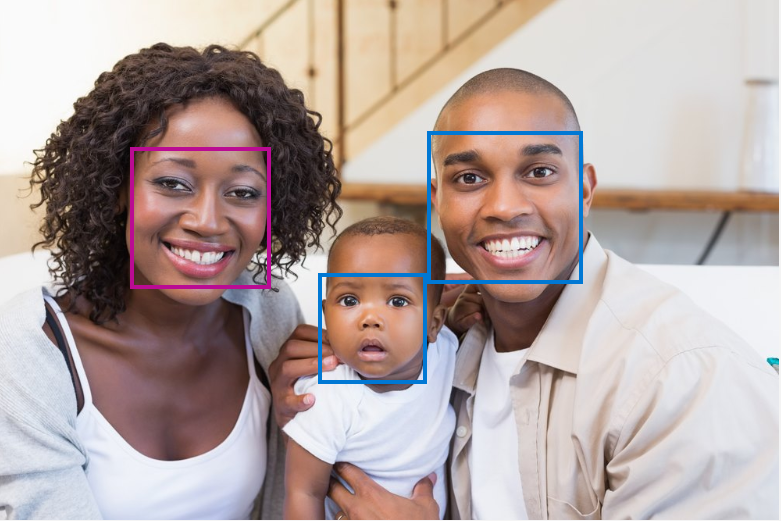
\includegraphics[width=\linewidth]{Face_recogn_micros_2.png}
	\caption{Cognitive services - Face recognition. Links de foto, rechts een JSON-file met herkende elementen.}
	\label{fig:cognitive2}
\end{figure}

\begin{figure}[h]
	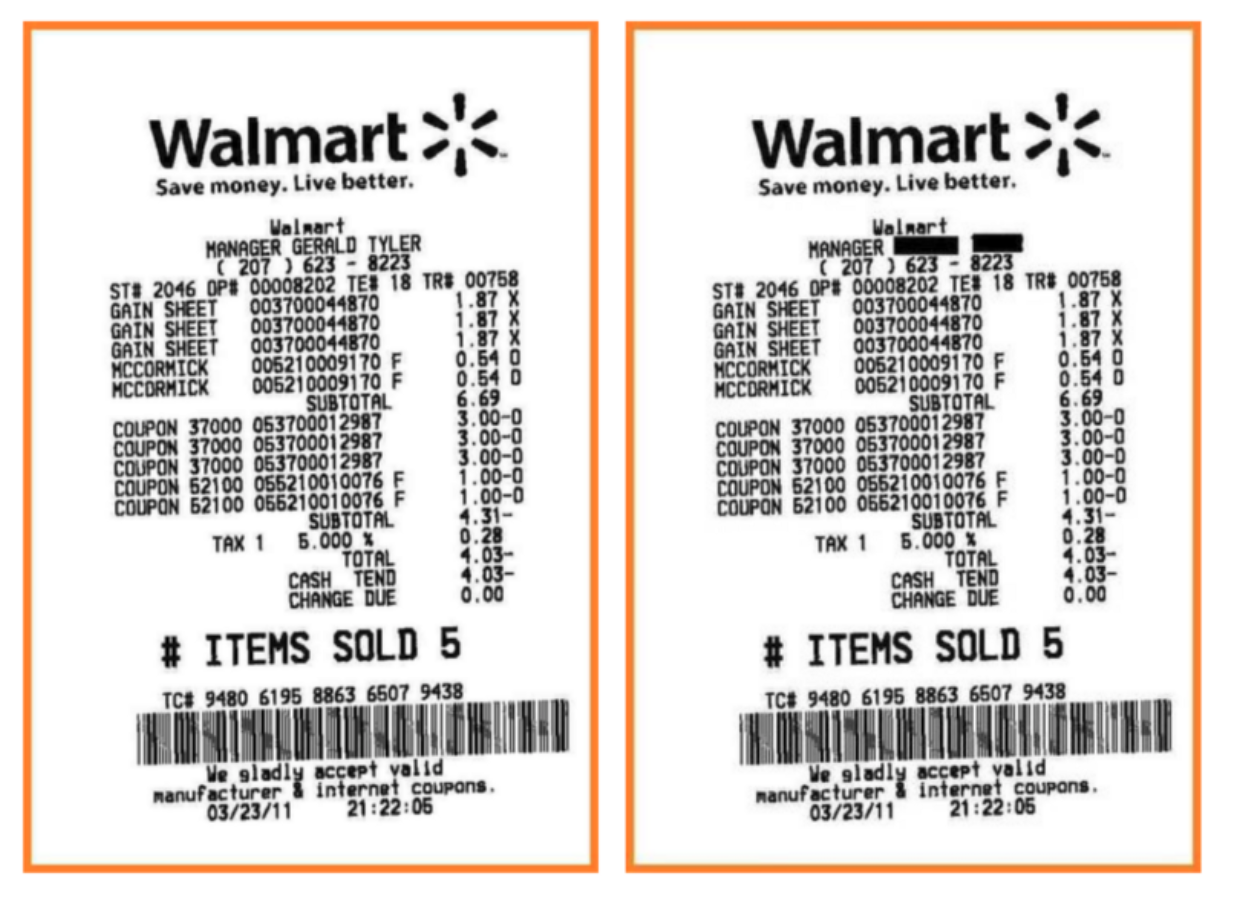
\includegraphics[width=\linewidth]{Receipt_name_covered.png}
	\caption{Cognitive services - Face recognition. Links de foto, rechts een JSON-file met herkende elementen.}
	\label{fig:receipt}
\end{figure}

[21-25]




https://gdpr-info.eu/recitals/ bijlage
Recital 26
1The principles of data protection should apply to any information concerning an identified or identifiable natural person. 2Personal data which have undergone pseudonymisation, which could be attributed to a natural person by the use of additional information should be considered to be information on an identifiable natural person. 3To determine whether a natural person is identifiable, account should be taken of all the means reasonably likely to be used, such as singling out, either by the controller or by another person to identify the natural person directly or indirectly. 4To ascertain whether means are reasonably likely to be used to identify the natural person, account should be taken of all objective factors, such as the costs of and the amount of time required for identification, taking into consideration the available technology at the time of the processing and technological developments. 5The principles of data protection should therefore not apply to anonymous information, namely information which does not relate to an identified or identifiable natural person or to personal data rendered anonymous in such a manner that the data subject is not or no longer identifiable. 6This Regulation does not therefore concern the processing of such anonymous information, including for statistical or research purposes.

Grond 75
EU-AVG
(75) Het qua waarschijnlijkheid en ernst uiteenlopende risico voor de rechten en vrijheden van natuurlijke personenkan voortvloeien uit persoonsgegevensverwerking die kan resulteren in ernstige lichamelijke, materiële of immateriële schade, met name: waar de verwerking kan leiden tot discriminatie, identiteitsdiefstal of -fraude, financiële verliezen, reputatieschade, verlies van vertrouwelijkheid van door het beroepsgeheim beschermde persoonsgegevens, ongeoorloofde ongedaanmaking van pseudonimisering, of enig ander aanzienlijk economisch of maatschappelijk nadeel; wanneer de betrokkenen hun rechten en vrijheden niet kunnen uitoefenen of worden verhinderd controle over hun persoonsgegevens uit te oefenen; wanneer persoonsgegevens worden verwerkt waaruit ras of etnische afkomst, politieke opvattingen, religie of levensbeschouwelijke overtuigingen, of vakbondslidmaatschap blijkt, en bij de verwerking van genetische gegevens of gegevens over gezondheid of seksueel gedrag of strafrechtelijke veroordelingen en strafbare feiten of daarmee verband houdende veiligheidsmaatregelen; wanneer persoonlijke aspecten worden geëvalueerd, om met name beroepsprestaties, economische situatie, gezondheid, persoonlijke voorkeuren of interesses, betrouwbaarheid of gedrag, locatie of verplaatsingen te analyseren of te voorspellen, teneinde persoonlijke profielen op te stellen of te gebruiken; wanneer persoonsgegevens van kwetsbare natuurlijke personen, met name van kinderen, worden verwerkt; of wanneer de verwerking een grote hoeveelheid persoonsgegevens betreft en gevolgen heeft voor een groot aantal betrokkenen.